\documentclass{beamer}
\mode<presentation>
\usepackage{amsmath}
\usepackage{amssymb}
%\usepackage{advdate}
\usepackage{adjustbox}
\usepackage{subcaption}
\usepackage{enumitem}
\usepackage{multicol}
\usepackage{mathtools}
\usepackage{listings}
\usepackage{float}
\usepackage{graphicx}
\usepackage{url}
\def\UrlBreaks{\do\/\do-}
\usetheme{Boadilla}
\usecolortheme{lily}
\setbeamertemplate{footline}
{
  \leavevmode%
  \hbox{%
  \begin{beamercolorbox}[wd=\paperwidth,ht=2.25ex,dp=1ex,right]{author in head/foot}%
    \insertframenumber{} / \inserttotalframenumber\hspace*{2ex} 
  \end{beamercolorbox}}%
  \vskip0pt%
}
\setbeamertemplate{navigation symbols}{}

\providecommand{\nCr}[2]{\,^{#1}C_{#2}} % nCr
\providecommand{\nPr}[2]{\,^{#1}P_{#2}} % nPr
\providecommand{\mbf}{\mathbf}
\providecommand{\pr}[1]{\ensuremath{\Pr\left(#1\right)}}
\providecommand{\qfunc}[1]{\ensuremath{Q\left(#1\right)}}
\providecommand{\sbrak}[1]{\ensuremath{{}\left[#1\right]}}
\providecommand{\lsbrak}[1]{\ensuremath{{}\left[#1\right.}}
\providecommand{\rsbrak}[1]{\ensuremath{{}\left.#1\right]}}
\providecommand{\brak}[1]{\ensuremath{\left(#1\right)}}
\providecommand{\lbrak}[1]{\ensuremath{\left(#1\right.}}
\providecommand{\rbrak}[1]{\ensuremath{\left.#1\right)}}
\providecommand{\cbrak}[1]{\ensuremath{\left\{#1\right\}}}
\providecommand{\lcbrak}[1]{\ensuremath{\left\{#1\right.}}
\providecommand{\rcbrak}[1]{\ensuremath{\left.#1\right\}}}
\theoremstyle{remark}
\newtheorem{rem}{Remark}
\newcommand{\sgn}{\mathop{\mathrm{sgn}}}
\providecommand{\abs}[1]{\left\vert#1\right\vert}
\providecommand{\res}[1]{\Res\displaylimits_{#1}} 
\providecommand{\norm}[1]{\lVert#1\rVert}
\providecommand{\mtx}[1]{\mathbf{#1}}
\providecommand{\mean}[1]{E\left[ #1 \right]}
\providecommand{\fourier}{\overset{\mathcal{F}}{ \rightleftharpoons}}
%\providecommand{\hilbert}{\overset{\mathcal{H}}{ \rightleftharpoons}}
\providecommand{\system}{\overset{\mathcal{H}}{ \longleftrightarrow}}
	%\newcommand{\solution}[2]{\textbf{Solution:}{#1}}
%\newcommand{\solution}{\noindent \textbf{Solution: }}
\providecommand{\dec}[2]{\ensuremath{\overset{#1}{\underset{#2}{\gtrless}}}}
\newcommand{\myvec}[1]{\ensuremath{\begin{pmatrix}#1\end{pmatrix}}}
\let\vec\mathbf

\lstset{
language=C,
frame=single, 
breaklines=true,
columns=fullflexible
}

\numberwithin{equation}{section}

\title{Presentation - Matgeo}
\author{Aryansingh Sonaye \\
AI25BTECH11032 \\
EE1030 - Matrix Theory}

\date{\today} 
\begin{document}

\begin{frame}
\titlepage
\end{frame}

\section{Problem}
\begin{frame}
\frametitle{Problem Statement}
\textbf{Problem 12.318}
Let $V$ be the vector space of all real polynomials of degree at most $20$. 
Define the subspaces
\begin{align}
W_1 = \{ p \in V : p(1)=p(\tfrac12)=p(5)=p(7)=0 \}, \\
W_2 = \{ p \in V : p(\tfrac12)=p(3)=p(4)=p(7)=0 \}.
\end{align}
Find $\dim(W_1 \cap W_2)$ .


\end{frame}

\section{Solution}
\subsection{Description of Variables used}
\begin{frame}
\frametitle{Description of Variables used}
\begin{table}[H]
\centering
\begin{tabular}{|c|c|}
\hline
Symbol & Description \\
\hline
$p(x)$ & Polynomial of degree $\leq 20$ \\
$c_i$ & Coefficients of $p(x)$ \\
$a$ & Point of evaluation (root condition) \\
$A$ & Constraint matrix from evaluations \\
\hline
\end{tabular}
\caption{} \label{}
\end{table}


\end{frame}

\subsection{Theoretical Solution }
\begin{frame}
\frametitle{Theoretical Solution}
\textbf{Definitions}

\textbf{Vector Space:}  
A set $V$ together with two operations (vector addition and scalar multiplication) is called a vector space over the field $\mathbb{R}$ if for all $\vec{u},\vec{v},\vec{w} \in V$ and scalars $a,b \in \mathbb{R}$, the following conditions hold:
\begin{itemize}
    \item Closure under addition: $\vec{u}+\vec{v} \in V$.
    \item Commutativity: $\vec{u}+\vec{v} = \vec{v}+\vec{u}$.
    \item Associativity: $(\vec{u}+\vec{v})+\vec{w} = \vec{u}+(\vec{v}+\vec{w})$.
    \item Existence of zero vector: $\exists \, \vec{0} \in V$ such that $\vec{u}+\vec{0}=\vec{u}$.
    \item Existence of additive inverse: $\forall \vec{u}\in V, \, \exists (-\vec{u}) \in V$ such that $\vec{u}+(-\vec{u})=\vec{0}$.
    \item Closure under scalar multiplication: $a\vec{u} \in V$.
    \item Distributivity: $a(\vec{u}+\vec{v}) = a\vec{u}+a\vec{v}$ and $(a+b)\vec{u}=a\vec{u}+b\vec{u}$.
    \item Compatibility: $a(b\vec{u})=(ab)\vec{u}$.
    \item Identity: $1\cdot \vec{u}=\vec{u}$.
\end{itemize}


\end{frame}

\begin{frame}
\frametitle{Theoretical Solution}
A subset $W \subseteq V$ is called a subspace of $V$ if:
\begin{itemize}
    \item $\vec{0} \in W$ (contains the zero vector),
    \item If $\vec{u},\vec{v}\in W$, then $\vec{u}+\vec{v}\in W$ (closed under addition),
    \item If $\vec{u}\in W$ and $\alpha \in \mathbb{R}$, then $\alpha \vec{u} \in W$ (closed under scalar multiplication).
\end{itemize}

\textbf{Dimension of a Subspace:}  
The dimension of a subspace $W$ of $V$ is the number of vectors in a basis of $W$, i.e.,
\[
\dim(W) = \text{number of linearly independent vectors that span } W.
\]


\end{frame}

\begin{frame}
\frametitle{Theoretical Solution}
\noindent
Step 1: Represent the polynomial
\begin{align}
p(x) &= c_0 + c_1x + c_2x^2 + \cdots + c_{20}x^{20}, \\
\vec{c} &= \myvec{c_0 \\ c_1 \\ \vdots \\ c_{20}} \in \mathbb{R}^{21}.
\end{align}

\noindent
Step 2: Each condition $p(a)=0$ gives
\begin{align}
p(a) &= \myvec{1 & a & a^2 & \cdots & a^{20}} \vec{c} = 0.
\end{align}

\noindent
Step 3: For the intersection $W_1 \cap W_2$, the polynomial must vanish at 
\[
\{1,\tfrac12,5,7,3,4\}.
\]

\end{frame}

\begin{frame}
\frametitle{Theoretical Solution}
Thus we obtain the matrix equation
\begin{align}
A \vec{c} &= \vec{0}, \quad \text{where} \\
A &= \myvec{
1 & 1 & 1^2 & \cdots & 1^{20} \\
1 & \tfrac12 & (\tfrac12)^2 & \cdots & (\tfrac12)^{20} \\
1 & 5 & 5^2 & \cdots & 5^{20} \\
1 & 7 & 7^2 & \cdots & 7^{20} \\
1 & 3 & 3^2 & \cdots & 3^{20} \\
1 & 4 & 4^2 & \cdots & 4^{20}
}.
\end{align}

\noindent
Step 4: The system $A\vec{c}=\vec{0}$ is a homogeneous system with $21$ unknowns 
and $6$ independent equations. Hence the number of free variables is
\begin{align}
21 - 6 = 15.
\end{align}

\noindent
\textbf{Final Answer:}
\begin{align}
\dim(W_1 \cap W_2) = 15
\end{align}
\end{frame}


\subsection{Plot}
\begin{frame}
    \frametitle{Plot}
\begin{figure}[H]
   \centering
   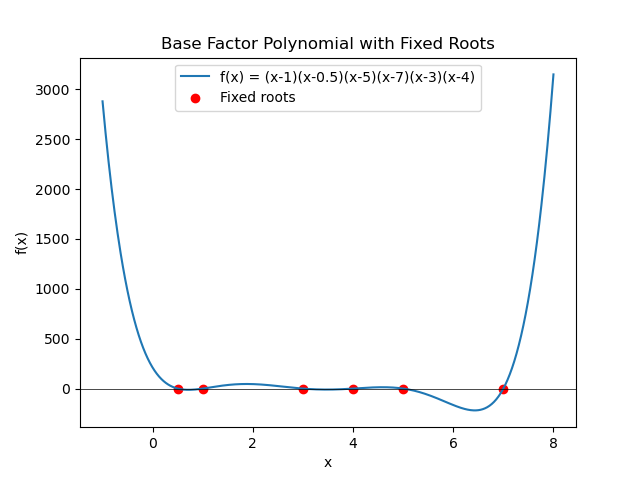
\includegraphics[width=0.8\columnwidth]{figs/poly_dim.png}
   \caption{}
   \label{}
   \end{figure}
\end{frame}

\begin{frame}[fragile]
    \frametitle{Code - C}
    \begin{lstlisting}
#include <stdio.h>

// Base factor polynomial f(x) = (x-1)(x-0.5)(x-5)(x-7)(x-3)(x-4)
double base_factor(double x) {
    return (x-1.0)*(x-0.5)*(x-5.0)*(x-7.0)*(x-3.0)*(x-4.0);
}



    \end{lstlisting}
    \end{frame}


\begin{frame}[fragile]
    \frametitle{Code - Python(with shared C code)}
    The code to obtain the required plot is
    \begin{lstlisting}
import ctypes
import numpy as np
import matplotlib.pyplot as plt

# Load the compiled C library
lib = ctypes.CDLL("./poly.so")
lib.base_factor.restype = ctypes.c_double

# Define a Python wrapper around the C function
def f(x):
    return lib.base_factor(ctypes.c_double(x))

# Generate values
xs = np.linspace(-1, 8, 600)
ys = [f(x) for x in xs]


\end{lstlisting}
\end{frame}
\begin{frame}[fragile]
\frametitle{Code - Python(with shared C code)}
\begin{lstlisting}
# Known fixed roots
roots = np.array([1.0, 0.5, 5.0, 7.0, 3.0, 4.0])

# Plot
plt.plot(xs, ys, label="f(x) = (x-1)(x-0.5)(x-5)(x-7)(x-3)(x-4)")
plt.scatter(roots, np.zeros_like(roots), color="red", label="Fixed roots")
plt.axhline(0, color="black", linewidth=0.5)
plt.xlabel("x")
plt.ylabel("f(x)")
plt.title("Base Factor Polynomial with Fixed Roots")
plt.legend()
plt.savefig("poly_dim.png")
plt.show()


\end{lstlisting}
\end{frame}

\begin{frame}[fragile]
\frametitle{Code - Python only}
\begin{lstlisting}
import numpy as np
import matplotlib.pyplot as plt

# Define the base factor polynomial
def f(x):
    return (x-1.0)*(x-0.5)*(x-5.0)*(x-7.0)*(x-3.0)*(x-4.0)

# Range of x values
xs = np.linspace(-1, 8, 600)
ys = f(xs)

# The six fixed roots
roots = np.array([1.0, 0.5, 5.0, 7.0, 3.0, 4.0])

# Plot the curve
plt.plot(xs, ys, label="f(x) = (x-1)(x-0.5)(x-5)(x-7)(x-3)(x-4)")



\end{lstlisting}
\end{frame}

\begin{frame}[fragile]
\frametitle{Code - Python only}
\begin{lstlisting}
# Mark the roots on the x-axis
plt.scatter(roots, np.zeros_like(roots), color="red", zorder=5, label="Fixed roots")

# Draw x-axis
plt.axhline(0, color="black", linewidth=0.8)

# Labels and title
plt.xlabel("x")
plt.ylabel("f(x)")
plt.title("Base Factor Polynomial with Fixed Roots")
plt.legend()
plt.savefig("new_poly_dim.png")
plt.show()

\end{lstlisting}
\end{frame}

\end{document}
